\documentclass[a4paper,11pt]{article}
\usepackage{graphicx}
\usepackage{epstopdf}
\graphicspath{ {../} }

\begin{document}
\title{Lab3 Report}
\author{Kailean O'Keefe}
\date{\today}
\maketitle

\section*{Introduction}
This lab explored the way that TCP manages how many bytes are in flight on a connection while transferring files as bytes across a network. It went in depth into which methods TCP uses to control the cwnd, as well as what TCP does to handle recovering from when a packet is dropped. 

\section*{TCP Tahoe}
The main implement of TCP explored in this lab was TCP Tahoe. In TCP Tahoe TCP uses the method of slow-start to ramp up to speed. Once a certain threshold is reached, Tahoe then uses congestion control to avoid clogging the connection. When a packet is dropped, Tahoe sets the threshold to half of the current cwnd and then resets the cwnd to 1 and begins transferring again using slow-start.

\pagebreak

\subsection{graph-0drop}
This is the first of 4 tests using TCP Tahoe. As shown by the graph below, when no packets are dropped, the cwnd window grows rather quickly before hitting the threshold and proceeding to grow linearly. Because no packets are dropped, cwnd would continue to grow indefinitely.

\begin{center}
\includegraphics[width=\linewidth]{graphs-0drop/cwnd}
\end{center}

\pagebreak

\subsection{graph-1drop}
In this section one packet is allowed to drop. This is reflected in the graph as we see the cwnd drop back down to 1 after about one second. The cwnd then grows until reaching the new threshold at around 7500 bytes and then continues to grow linearly after that point. 

\begin{center}
\includegraphics[width=\linewidth]{graphs-1drop/cwnd}
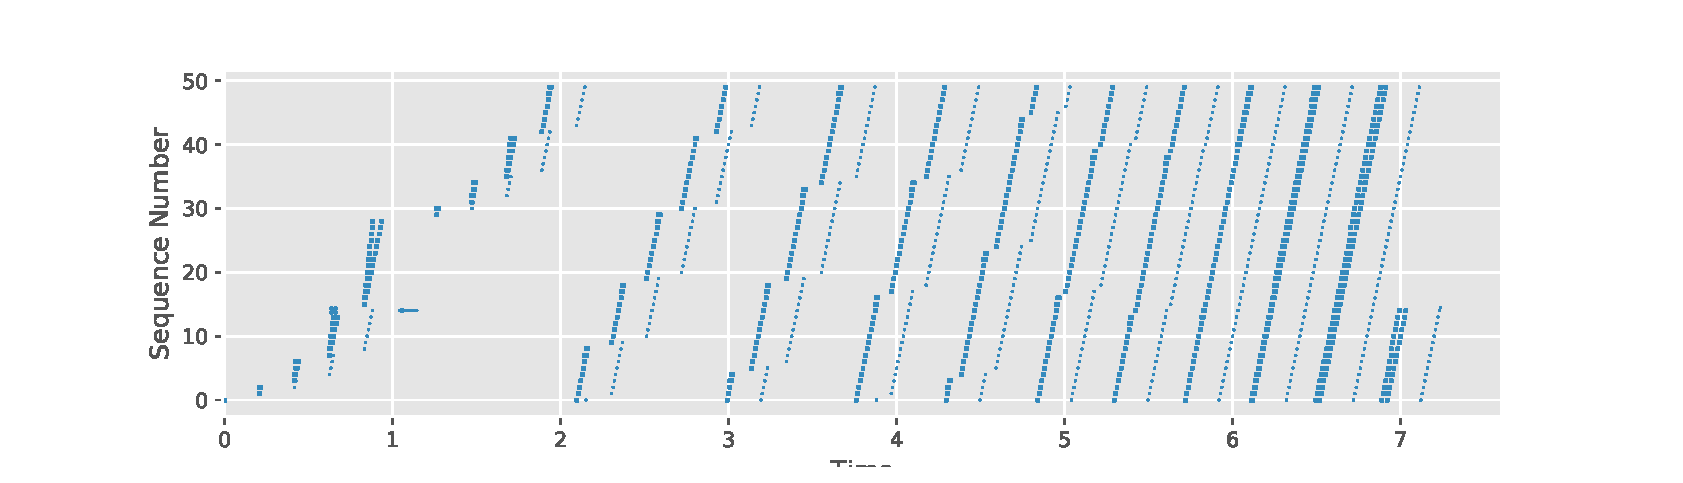
\includegraphics[width=\linewidth]{graphs-1drop/sequence}
\end{center}

\pagebreak

\subsection{graph-2drop}
This section looks identical to the previous section due to the fact that the packets are dropped so close to one another. 

\begin{center}
\includegraphics[width=\linewidth]{graphs-2drop/cwnd}
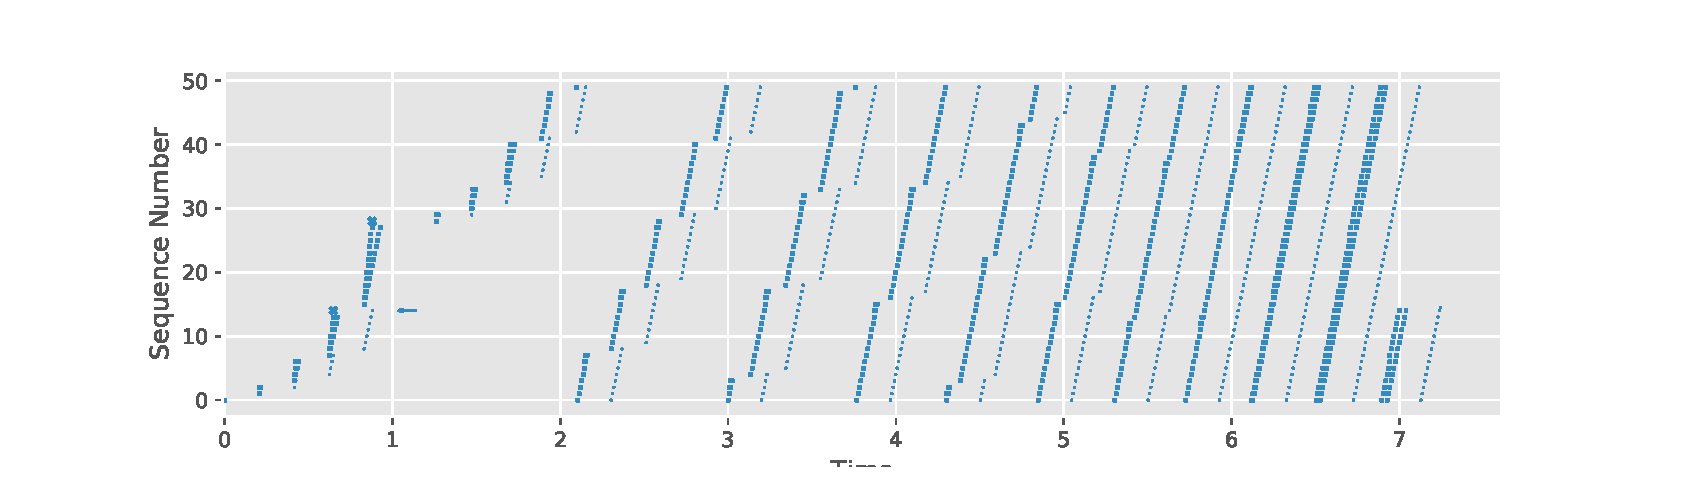
\includegraphics[width=\linewidth]{graphs-2drop/sequence}
\end{center}

\pagebreak

\subsection{graph-3drop}
In this section 3 packets were dropped on the connection. While the graphs for this section look very similar to sections 1 and 2, if you look closely you will notice that there are in fact some subtile differences between them. In the 3 graph we notice that the amount of packets dropping has led to congestion avoidance being applied much more between seconds 1 and 2 than in the previous graphs. 

\begin{center}
\includegraphics[width=\linewidth]{graphs-3drop/cwnd}
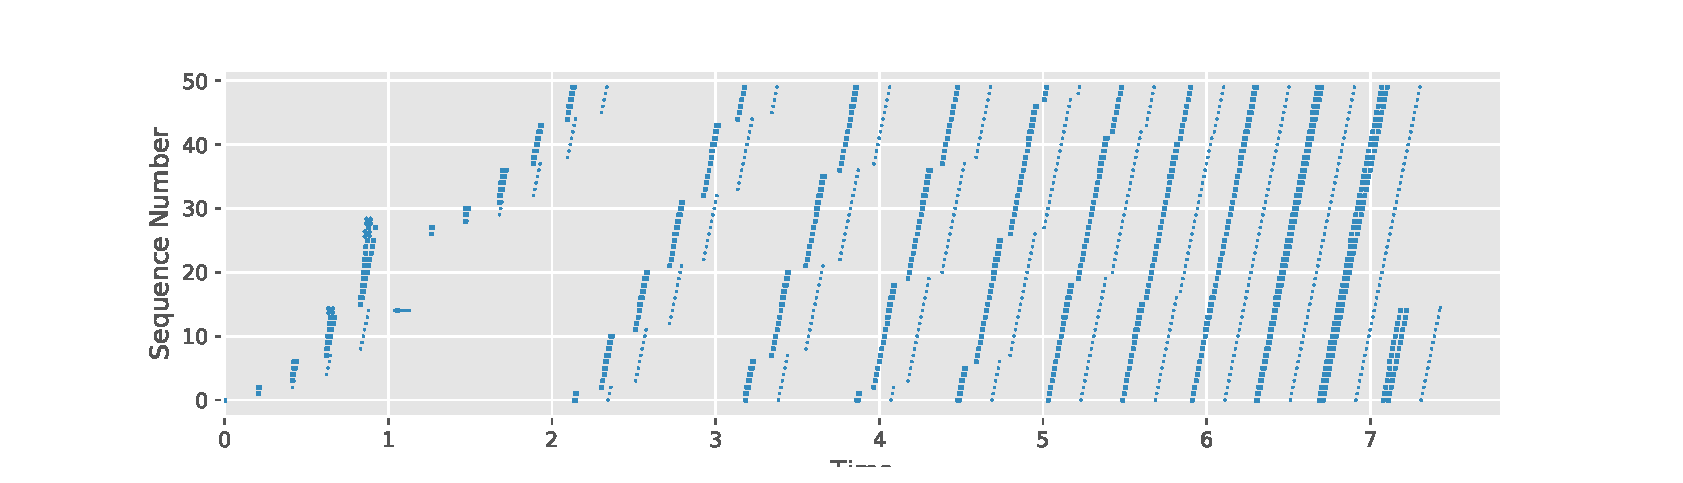
\includegraphics[width=\linewidth]{graphs-3drop/sequence}
\end{center}

\pagebreak

\section*{Conclusion}
This lab has given us a firm understanding of the way that TCP Tahoe is able to regulate the amount of data being transferred over a connection. It iterates the importance of having a stable connection when sending data, but also shows how an application can quickly recover when data is lost. 
\end{document}
